\addtocontents{toc}{\protect\addvspace{5pt}}
\chapter{METODE PENELITIAN}

\section{Tempat dan Waktu Penelitian}
Penelitian "Optimasi Model \emph{Physics-Informed Neural Networks} untuk Menyelesaikan Persamaan Schrodinger Non-Linear dalam Analisis Perambatan Pulsa Fiber Optik" dilakukan pada Bulan Februari hingga Mei 2025 pada Laboratorium Fisika Komputasi, Jurusan Fisika, Fakultas MIPA, Universitas Brawijaya menggunakan fasilitas AI Center Universitas Brawijaya.

\section{Alat dan Bahan}
Penelitian dilakukan menggunakan \emph{Jupyter Notebook} pada fasilitas \emph{super computer} NVIDIA seri DGX A100 yang disediakan oleh AI Center Universitas Brawijaya. Bahasa pemrograman Python digunakan dengan didukung oleh beberapa pustaka dalam implementasi dan analisis algoritma PINNs. Beberapa pustaka utama yang digunakan meliputi:

\begin{table}[htbp]
    \centering
    \begin{threeparttable}
        \caption{Daftar Pustaka yang Digunakan}
        \begin{tabular}{|p{2cm}|p{8cm}|}
				\hline
				Pustaka & Informasi \\
                \hline 
                \textbf{Pytorch} & Pustaka khusus dalam pembangunan arsitektur akal imitasi PINNs dan optimasi model melalui diferensiasi otomatis.\\
                \hline
                \textbf{Numpy} & Pustaka yang digunakan dalam operasi aljabar linear dan manipulasi array dalam persiapan data.\\
                \hline
                \textbf{Matplotlib} & Pustaka yang digunakan dalam visualisasi perambatan pulsa dan analisis data PINNs.\\
                \hline
                \textbf{Scipy} & Pustaka matematika yang diimplementasikan pada metode SSFM.\\
                \hline
			\end{tabular}
    \end{threeparttable}
\end{table} 

\section{Desain Penelitian}
Penelitian dilakukan dengan pendekatan kuantitatif komputasional untuk mengevaluasi kemampuan generalisasi PINNs dalam menyelesaikan Persamaan Non-Linear Schr\"odinger pada sistem \emph{ultrashort pulse} berdasarkan persamaan \eqref{governing-equation3}.

\begin{align}
    \label{governing-equation3}
    \frac{\partial A(t,z)}{\partial z}
    &+ \frac{\alpha}{2} A(t,z) 
    + i \frac{\beta_2}{2} \frac{\partial^2 A(t,z)}{\partial t^2} \notag \\
    &-  \frac{\beta_3}{6} \frac{\partial^3 A(t,z)}{\partial t^3} 
    - i \gamma |A(t,z)|^2 A(t,z) 
    = 0
\end{align}

Kondisi awal sistem diberikan berdasarkan persamaan secant hiperbolik $A(t,0) = A_0 \frac{1}{\cosh(t/T_0)}$ di mana $A_0$ menyatakan amplitudo pulsa awal dan $T_0$ menyatakan lebar pulsa. Parameter persamaan NLS diberikan pada tabel di bawah:

\begin{table}[htbp]
    \centering
    \begin{threeparttable}
        \caption{Parameter pada Persamaan NLS}
        \label{TabelParam}
        \begin{tabular}{|c|c|}
            \hline
            \textbf{Parameter} & \textbf{Nilai} \\
            \hline
            $\alpha$ & 0.5 dB/m \\
            \hline
            $\beta_2$ & $-5.23 \times 10^{-27}$ s$^2$/m \\
            \hline
            $\beta_3$ & $4.27 \times 10^{-41}$ s$^3$/m \\
            \hline
            $\gamma$ & $18.4 \times 10^{-3}$ W$^{-1}$m$^{-1}$ \\
            \hline
            lebar pulsa ($l$) & $0.58 \times 10^{-12}$ ps \\
            \hline
            amplitudo ($A_0$) & $\sqrt{22.04} \text{W}^{1/2}$ \\
            \hline
            Domain $T$ & $[-1.4 \times 10^{-12},\ 1.4 \times 10^{-12}]$ s \\
            \hline
            Domain $Z$ & $[0,\ 11]$ m \\
            \hline
        \end{tabular}
    \end{threeparttable}
\end{table}

Dalam penelitian ini, selain menyelesaikan persamaan \eqref{governing-equation3} menggunakan model dasar PINNs (selanjutnya disebut sebagai Vanilla-PINNs), turut dirancang modifikasi model PINNs melalui penambahan sampel adaptif. Modifikasi ini diperkenalkan sebagai \emph{SMOTE-Adaptive-Sampling PINNs} (SAS-PINNs). Modifikasi ini mengimplementasikan teknik SMOTE untuk menambahkan titik kolokasi pada daerah yang sulit dipelajari oleh model. Data sampel kolokasi diidentifikasi dan dikelompokkan berdasarkan nilai residu. Sebagian dari data dengan nilai residu tertinggi diperlakukan sebagai kelas minoritas sementara sisanya dianggap sebagai kelas mayoritas. Titik kolokasi pada kelas minoritas kemudian dilakukan \emph{oversampling} menggunakan SMOTE sehingga mencapai target tertentu. Strategi ini dirancang untuk mempermudah konvergensi pada kawasan domain di mana model mengalami kesulitan.

\begin{figure}[htbp]
    \centering
    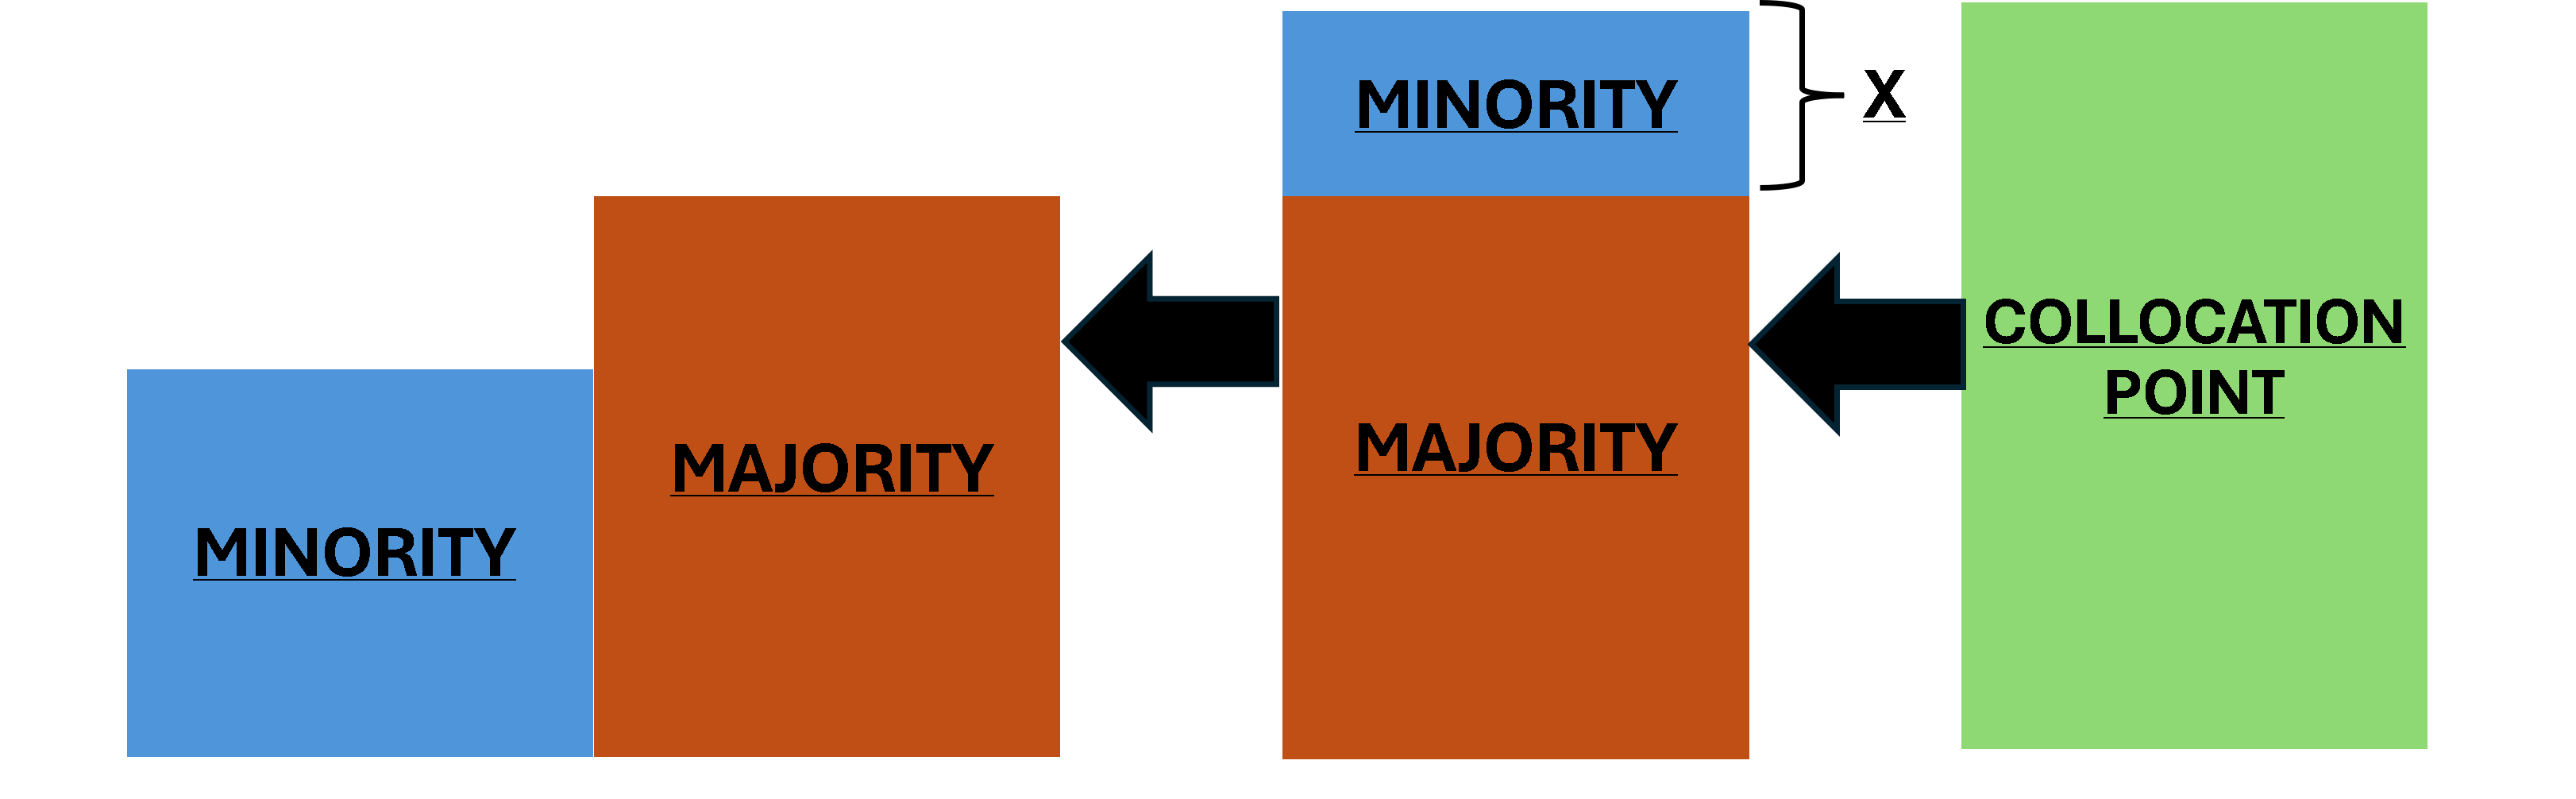
\includegraphics[width=0.8\linewidth]{Gambar/SAS-PINNs-TR.png}
    \caption{Visualisasi Penambahan Sampel SAS-PINNs} 
    \label{fig:SASviz}
\end{figure}

Dalam konfigurasi SAS-PINNs, diperkenalkan dua parameter tambahan berupa Nilai Ambang dan Rasio \emph{Oversampling}. Nilai Ambang menyatakan bagian dari keseluruhan titik kolokasi (dalam desimal) dengan nilai residu tertinggi yang diperlakukan sebagai minoritas. Jumlah nilai ambang tidak dapat melebihi 0.5, atau setengah dari jumlah titik kolokasi. Rasio \emph{oversampling} menyatakan rasio dari jumlah target kelompok minoritas setelah dilakukan penambahan data terhadap kelompok mayoritas.

Evaluasi model dilakukan dengan membandingkan masing-masing model pada tiap perlakuan menggunakan nilai referensi. Nilai referensi ini diperoleh berdasarkan pendekatan numerik SSFM. Parameter evaluasi meliputi akurasi prediksi model terhadap nilai referensi dan kepresisian prediksi model pada beberapa uji ulang. 
\newpage 
\section{Prosedur Penelitian}

Prosedur penelitian diberikan dalam flowchart berikut:

\begin{figure}[htbp]
    \centering
    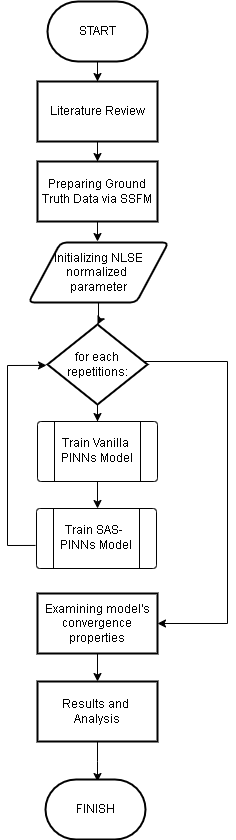
\includegraphics[width=0.32\linewidth]{Gambar/FlowchartFix.png}
    \caption{Flowchart Penelitian} 
    \label{fig:main-flowchart}
\end{figure}

\newpage
Peninjauan pustaka dilakukan untuk mendapatkan informasi terkait yang diperlukan dalam penelitian. Selanjutnya, data referensi disintesis atas validasi prediksi PINNs menggunakan SSFM. Parameter ternormalisasi kemudian diinisialisasi sebelum proses pembelajaran PINNs dilakukan. Pembelajaran dilakukan menggunakan struktur jaringan neural Vanilla-PINNs dan SAS-PINNs. Sifat konvergensi model dianalisis dan dibandingkan satu sama lain berdasarkan nilai error model dan presisi pada beberapa uji ulang. 


\subsection{Sintesis Data Referensi Melalui SSFM}
Data referensi diperlukan sebagai validasi atas prediksi PINNs. Data ini disusun menggunakan SSFM sebagai metode yang umum digunakan dalam menyelesaikan persamaan NLS. Grid numerik SSFM diinisialisasi sebagai \(2^{11}\) \emph{timesteps} dan \(2^7\) \emph{lengthsteps}. Dengan demikian, dinamika propagasi pulsa memiliki resolusi yang cukup tinggi untuk dibandingkan dengan model PINNs. Flowchart dari SSFM diberikan pada Gambar \ref{fig:ssfm-flowchart}.

Operator nonlinear $\mathcal{N}$ dan linear $\mathcal{L}$ diberikan dalam persamaan \eqref{nonlinear3} dan \eqref{linear3}

\begin{equation}
    \hat{\mathcal{N}} = i\gamma dz
    \label{nonlinear3}
\end{equation}

\begin{equation}
    \hat{\mathcal{L}} = \exp\left( i\frac{\beta_2}{2\omega^2}-i\frac{\beta_3}{6\omega^3} -\alpha/2 \right)dz
    \label{linear3}
\end{equation}

Penyelesaian operator nonlinear dan linear diberikan dalam persamaan \eqref{nonlinear-step} dan \eqref{linear-step} sebagai: 

\begin{equation}
    A_N(t,z+dz) = A(t,z)\exp(\hat{\mathcal{N}}|A|^2)
    \label{nonlinear-step}
\end{equation}

\begin{equation}
    A(t,z+dz) = \mathcal{F}^{-1}(\mathcal{F}(A_N)\hat{\mathcal{L}})
    \label{linear-step}
\end{equation}

\newpage
\begin{figure}[htbp]
    \centering
    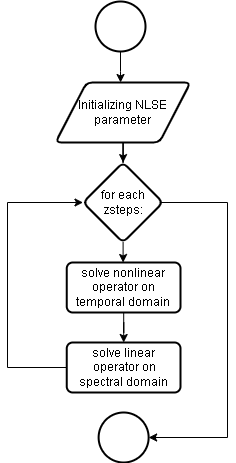
\includegraphics[width=0.4\linewidth]{Gambar/SSFM-F.png}
    \caption{Flowchart SSFM} 
    \label{fig:ssfm-flowchart}
\end{figure}


\subsection{Inisialisasi Parameter Persamaan NLS dalam PINNs}

Persamaan NLS didasarkan atas parameter Tabel \ref{TabelParam}. Nilai \(\alpha\) pada satuan dB perlu dikonversi ke Nepers dengan dikalikan \(\dfrac{\log(10)}{10}\). Selain itu normalisasi  perlu dilakukan pada fungsi \eqref{governing-equation3} dikarenakan skala nilai parameter yang terpaut jauh. Perbedaan ini berpotensi menyebabkan ketidakseimbangan pembelajaran PINNs. Normalisasi persamaan dilakukan dengan mengubah variabel $(t,z)$ menjadi unit satuan sebagai $(t,z) = (T\hat{t}, Z\hat{z})$ untuk meningkatkan stabilitas numerik dan mempercepat konvergensi pembelajaran. Maka dari itu, domain perambatan pulsa diatur sebagai $\hat{t} \in [-1,1]$ dan $\hat{z} \in [0,1]$. Persamaan diferensial ternormalisasi, dengan demikian, menjadi:

\begin{align}
    \mathcal{H} =\frac{\partial A(\hat{t},\hat{z})}{\partial \hat{z}}
    &+ \frac{\alpha Z}{2} A(\hat{t},\hat{z}) 
    + i \frac{\beta_2 Z}{2T^2} \frac{\partial^2 A(\hat{t},\hat{z})}{\partial \hat{t}^2} \notag \\
    &-  \frac{\beta_3 Z}{6T^3} \frac{\partial^3 A(\hat{t},\hat{z})}{\partial \hat{t}^3} 
    - i \gamma Z |A(\hat{t},\hat{z})|^2 A(\hat{t},\hat{z})
    \label{normalized-eq}
\end{align}
\subsection{Inisialisasi Model PINNs}

Model PINNs diinisialisasi sebagai jaringan neural dengan dua input (\(t,x\)), dua neuron output (\(u,v\)), dan empat lapisan tersembunyi, masing-masing berisi 128 neuron. Dua neuron input difungsikan untuk menerima dimensi temporal dan spasial model. Sementara itu, dua neuron output, masing-masing merepresentasikan bagian riil dan imajiner dari solusi persamaan. Setiap lapisan tersembunyi dilengkapi dengan fungsi aktivasi \(\tanh()\). 

Fungsi biaya PINNs tersusun oleh fungsi biaya residu dan fungsi biaya data berdasarkan prediksi kondisi awal dan syarat batas Dirichlet serta Neumann. Masing-masing fungsi biaya diberikan faktor pembobot untuk mengatur kontribusi dari masing-masing komponen. Bobot komponen untuk fungsi residual diatur dan syarat batas diatur sebagai 1, sementara fungsi biaya kondisi awal sebagai 10 oleh karena sensitivitas PINNs terhadap kondisi awal.

\begin{equation}
    \mathcal{L}_{total} = \lambda_{i}\mathcal{L}_{init}+\lambda_{r}\mathcal{L}_{residue}+\lambda_{b}\mathcal{L}_{bound}
    \label{total-loss}
\end{equation}

\noindent
Fungsi biaya residual $\mathcal{L}_{residue}$ diberikan sebagai: 

\begin{equation}
    \mathcal{L}_{residue} =  \sum_{d_i = 1}^{N_{\mathcal{H}}} \mathcal{H}_u^2+\mathcal{H}_v^2
\end{equation}

\noindent
Sementara itu, fungsi biaya syarat awal dinyatakan dengan: 

\begin{equation}
    \mathcal{L}_{init} =  \sum_{d_i = 1}^{N_{\mathcal{I}}} \bigg( (u_{init}-\bar{u}_{init})^2 + (v_{init}-\bar{v}_{init})^2 \bigg)
\end{equation}

\noindent 
dengan \(\bar{u}_{init}\) dan \(\bar{v}_{init}\) menyatakan pulsa riil dan imajiner yang diketahui.

\noindent
Syarat batas Dirichlet dan Neumann periodik diberikan pada persamaan. Syarat ini menyatakan simetri pada kedua ujung domain, $A(-1,z) = A(1,z)$ dan $$\frac{\partial}{\partial t}(-1,z) = \frac{\partial}{\partial t}A(1,z)$$

\begin{equation}
    \mathcal{L}_{boundD} =  \frac{1}{N_B}\sum_{d_i = 1}^{N_B} \left((u(1,z)-u(-1,z)^2 + (v(1,z)-v(-1,z))^2 \right)
\end{equation}

\begin{align}
\mathcal{L}_{boundN} 
&= \frac{1}{N_B} \sum_{d_i = 1}^{N_B} \Bigg[
    \left( \left.\frac{\partial u}{\partial t} \right|_{t = -1} - 
           \left.\frac{\partial u}{\partial t} \right|_{t = 1} \right)^2 
    \notag \\ &\quad
    + \left( \left.\frac{\partial v}{\partial t} \right|_{t =-1} - 
             \left.\frac{\partial v}{\partial t} \right|_{t = 1} \right)^2
\Bigg]
\end{align}

\begin{equation}
     \mathcal{L}_{bound} = \mathcal{L}_{boundN} + \mathcal{L}_{boundD}
\end{equation}

Model dioptimasi menggunakan strategi optimasi gabungan: ADAM selama 40000 epoch dan LBFGS selama 5000 epoch. Laju pembelajaran ADAM diatur sebesar \(10^{-4}\) dan berkurang sebanyak 10\% untuk tiap 5000 epoch. Pendekatan ini menggabungkan keunggulan dari kedua metode, dengan ADAM memberikan laju konvergensi yang cepat, sementara LBFGS memberikan presisi lebih tinggi pada tahap akhir pelatihan

\newpage
\subsection{Pembelajaran PINNs}

Pembelajaran PINNs terbagi atas tahapan pembelajaran Vanilla-PINNs dan SAS-PINNs dengan algoritma yang diberikan pada flowchart di bawah

\begin{figure}[htbp]
    \centering
    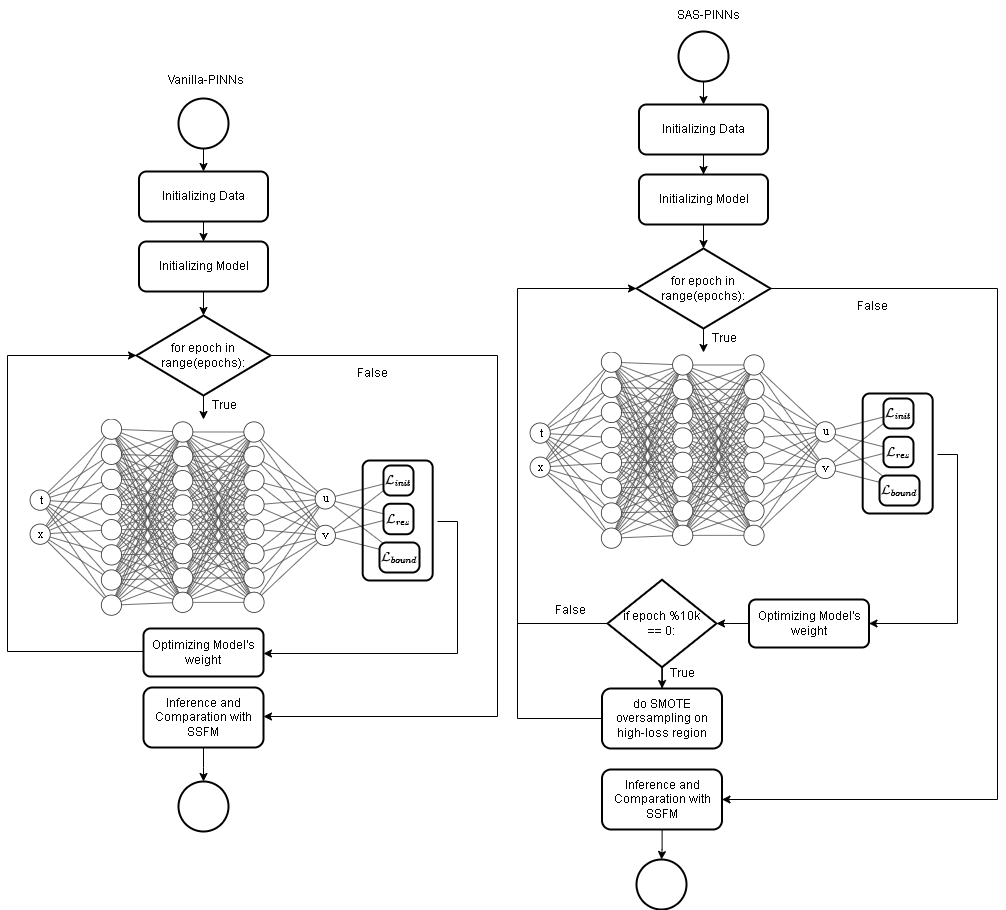
\includegraphics[width=1\linewidth]{Gambar/PINN-Diagram.png}
    \caption{Flowchart PINNs}
    (a) (kiri) Vanilla-PINNs; (b) (kanan) SAS-PINNs
    \label{fig:enter-label}
\end{figure}

Data yang diperlukan PINNs disampel menggunakan metode \emph{Latin Hypercube Sampling}. Jumlah sampel titik awal diberikan sebagai 500 dan titik batas sebagai 500 pada kedua sisi. Pada Vanilla-PINNs, jumlah titik kolokasi menjadi variabel bebas yang divariasikan pada [2.000, 5.000, 10.000, 20.000, dan 40.000]. Hal ini dilakukan untuk menilai bagaimana pengaruh jumlah sampel domain terhadap konvergensi PINNs. Proses pembelajaran PINNs pada tiap variasi jumlah sampel diulangi pada \emph{random seed} [0, 25, 420, 9999] untuk mendapatkan hasil yang lebih akurat. 

Pembelajaran SAS-PINNs dilakukan dengan jumlah sampel titik awal dan titik batas, serta struktur model dan strategi optimasi yang sama dengan model sebelumnya. Akan tetapi, jumlah titik kolokasi diatur tetap sejumlah 10.000. Konfigurasi nilai ambang dan rasio \emph{oversampling} ialah: 

\begin{table}[htbp]
    \centering
    \begin{threeparttable}
        \caption{Nilai Ambang dan Rasio SAS-PINNs}
        \begin{tabular}{|p{5cm}|p{4cm}|}
				\hline
				Nilai Ambang & Rasio \\
                \hline 
                0.45 & 1\\
                \hline
                0.35 & 0.7 \\
                \hline
                0.25 & 0.4 \\
                \hline
                0.15 & 0.25 \\
                \hline
			\end{tabular}
    \end{threeparttable}
\end{table} 

Pemilihan kedua parameter ini didasarkan atas jumlah data yang ditambahkan dan bagaimana data tersebut terdistribusi. Semakin kecil nilai ambang, data augmentasi SAS-PINNs semakin terfokus pada daerah dengan residu tertinggi. Namun, nilai ambang yang lebih besar mengakibatkan distribusi data yang lebih tersebar. Masing-masing konfigurasi SAS-PINNs dilakukan perulangan dengan empat \emph{random seed} yang sama dengan percobaan Vanilla-PINNs. Proses augmentasi titik kolokasi dilakukan untuk setiap 10000 \emph{epoch} dalam strategi optimasi ADAM. 


\subsection{Evaluasi Model}
Model dievaluasi berdasarkan akurasinya terhadap nilai referensi SSFM dan konsistensi prediksi model pada beberapa uji ulang untuk \emph{random seed yang berbeda}. Akurasi model diukur menggunakan metrik \emph{mean square error} (MSE). Presisi model diukur dengan mengamati persebaran nilai MSE dan rata-rata MSE model pada masing-masing perlakuan. 


\begin{equation}
    MSE = \frac{1}{N}\sum_{i=1}^N |A_i-\bar{A}_i|^2
\end{equation}

\noindent
nilai $A$ menyatakan prediksi pulsa kompleks PINNs, sementara $\bar{A}$ menyatakan pulsa referensi. 


